\section{Introduction}
\label{sec:introduction}

Where a pipeline's outputs are closed (classification labels, extraction
fields, retrieval hits), practice is settled: build a golden dataset, report
recall and precision, ship when the numbers clear the service threshold. A
golden dataset's real force is not that it stores correct answers but that it
holds the yardstick still: the same output scored twice gets the same
score. Open-output pipelines (agent transcripts, long-form generation, tool-use
traces) admit no such dataset; teams put an LLM judge in its place, and a judge
scoring the same output twice does not, in general, return the same number.
That is measured, not assumed: scored ten times over, several judges disagree
with themselves, and for most of them temperature zero does not settle it
\citep{lau2026sameinput}. This paper addresses the question that situation
forces: \emph{in open-output pipelines where no golden dataset can exist, what
licenses a verdict?}

\paragraph{Certify the instrument before trusting the reading.}
Before a factory trusts a gauge to accept or reject parts it measures how much
the gauge itself wobbles, and calls a part-to-part difference real only once it
exceeds that spread. We do the same for the LLM judge: measure its spread by
repeating it, and read a smallest resolvable difference off that. (Intuition
only; Section~\ref{sec:framework}'s definitions stand without it.)

Our answer is deliberately narrow. Failing our bar does not make a verdict
wrong; it breaks the link between the measurement and the claim, not the
judgment itself. A verdict far from its threshold survives an unsteady
yardstick; one near threshold, without margin, does not
(Section~\ref{sec:protocol} turns that margin into a table).
The lineage we borrow keeps two thresholds: detectable, and important
by an external criterion (Section~\ref{sec:related}); $\mdi$ is the first;
Contribution~5 measures the gap to the second.

We treat this as a problem of \emph{measurement rigor} in evaluation science,
and the field has asked for exactly that: \citet{bean2025construct} find only
$16\%$ of $445$ LLM benchmarks using uncertainty estimates or statistical
tests, \citet{apollo2024science} call for ``a science of evals,'' and
\citet{jiang2026itemlevel} want item-level results released rather than
discarded. We answer a small slice of it: the test--retest reliability of the
LLM judge, and what it implies for when an observed gain licenses a claim.

The acceptance side has begun to be addressed: a concurrent preprint
\citep{zayxshawn2026pace} gives an anytime-valid acceptance test for
accept-if-better rules and notes that its guarantee does not control
\emph{power}. That open side is what we take up. Type~I control asks whether a
claimed gain is real; we ask first whether the measurement can resolve a gain
of that size at all. This does not conflict with reinforcement
learning's tolerance of verifier noise \citep{plesner2026imperfect}: there
noise is redrawn each epoch and averaged over rollouts, while an
evaluation-gated pipeline sends the same noise through an accept-if-better
gate. Averaging cancels noise; selection amplifies it.

\begin{figure}[t]
  \centering
  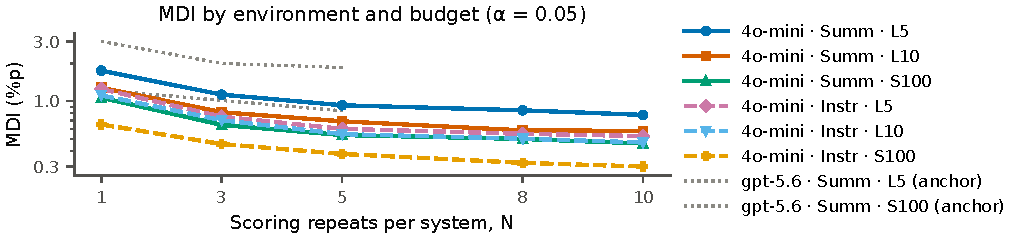
\includegraphics[width=\linewidth]{../figures/mdi_overlay_alpha0p05.pdf}
  \caption{The smallest gain an evaluation can separate from judge noise is not
    a constant: it depends on the environment ($2.7\times$ across the coloured
    dense tier at $N{=}1$) and on the budget $N$. Anchor curves (grey) use fewer
    items and repeats and are left out of that ratio; values in
    Table~\ref{tab:exp1-lookup}.}
  \label{fig:mdi-overview}
\end{figure}

\paragraph{Contributions.}
\begin{enumerate}
  \item \textbf{An $N$-dependent Minimum Detectable Improvement.} We
    formalize $\mdi(\env, N)$: a decision threshold expressed in observed
    score-difference units that is a function of the measurement budget $N$
    (scoring repeats). Prior work measures judge-level thresholds
    $\Delta^*(J)$ (cf.\ \citealp{usami2026darkcurrent}); where a repeat
    axis exists it counts calls to recover the judge's \emph{own} majority
    verdict \citep{yagubyan2026coinflip}; a detection threshold as a
    function of $(J, N)$ is unclaimed.
  \item \textbf{The False Improvement Probability, conditioned on the
    observed gain.} $\fip(\Delta, \env, N)$: the probability an observed
    gain $\Delta$ reverses under independent re-evaluation; conditioning
    on the \emph{observed} $\Delta$ is unclaimed in prior work.
  \item \textbf{A budget-indexed table of $\mdi$.} Per budget
    $N \in \{1,3,5,8,10\}$, the smallest gain each environment can separate
    from noise at level $\alpha$, with the stated multiplier to any target
    power, the Type~II side that acceptance testing leaves uncontrolled.
  \item \textbf{Noise-channel separation by a repeat sweep.} More scoring
    repeats make instability-driven gains vanish while a procedural
    component remains, which the sweep prices; clearing the threshold
    therefore rules out the instability channel alone, not judge bias
    (Section~\ref{sec:limitations}). We demonstrate the sweep on our grid
    and apply the promotion-time noise test it implies to a public
    improvement-loop trace released without repeats.
  \item \textbf{A measured boundary on what the threshold licenses.}
    Clearing $\mdi$ separates pairs on the judge's own scale while carrying
    almost no information about whether an expert reference agrees: it fires
    on pairs no annotation facet separates, and stays silent on one that
    three of four do (Section~\ref{sec:exp1}): the detectable/important
    pair's second threshold, measured rather than assumed.
\end{enumerate}

The measurements reported here are pilot-scale (direction, not final
precision), and every quantitative claim in the paper obeys the protocol it
proposes (Section~\ref{sec:protocol}).
